 \section{Actividad – Cálculos} 
Para crear los informes en Power BI Desktop, primero debe conectarse a los datos y después darles forma. Después podrá guardar los informes en el formato de archivos de Power BI Desktop, que es la extensión .pbix. Y también va a poder compartirlos. Puede hacerlo como cualquier otro archivo, pero sin duda como va a aprovechar todo su potencial será si lo comparte desde el servicio de Power Bi.
\begin{itemize}
	\item Conectarse a datos: normalmente son varios orígenes de datos.
	\item Dar forma a dichos datos: mediante las consultas que crean modelos de datos precisos.
	\item Crear informes: usando modelos que otros pueden aprovechar, compartir y usar como punto de partida.\\
\end{itemize} 

\begin{itemize}
	\item Resultado de cálculos en PowerBI
	\begin{center}
	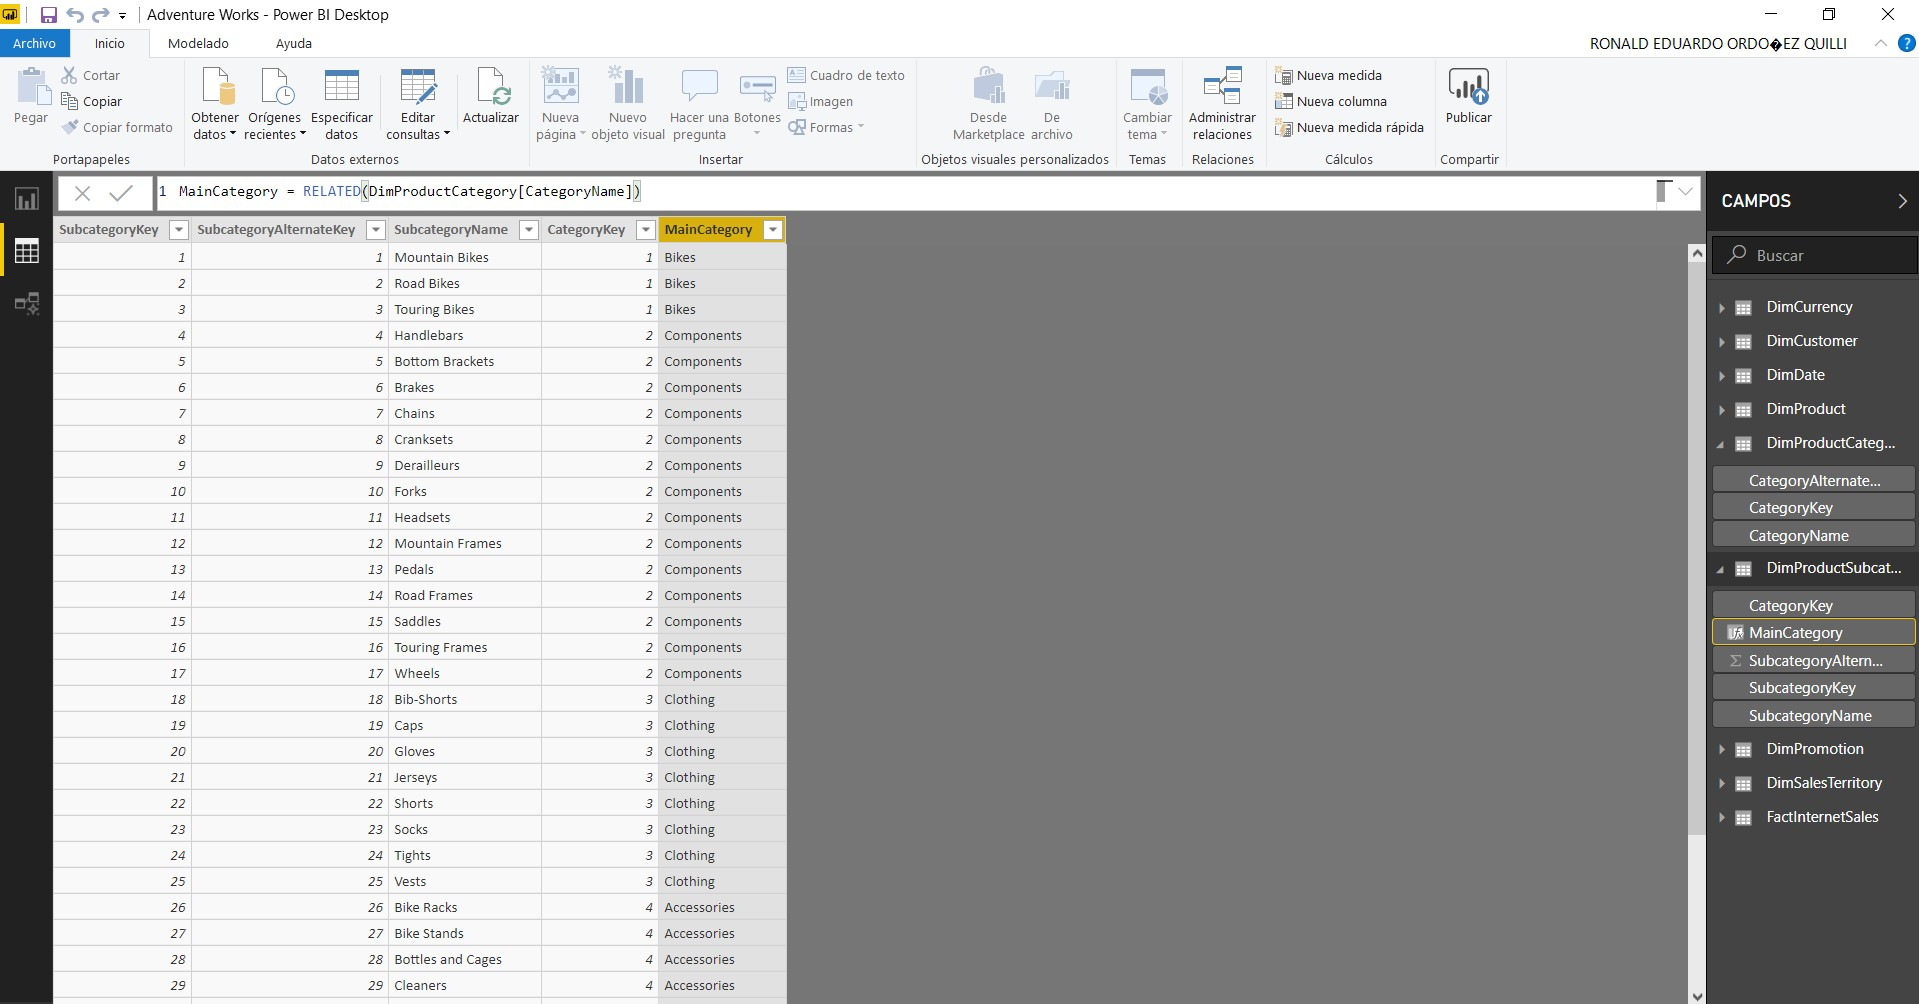
\includegraphics[width=16cm]{./Imagenes/imgpbi3} 
	\end{center}
	\begin{center}
	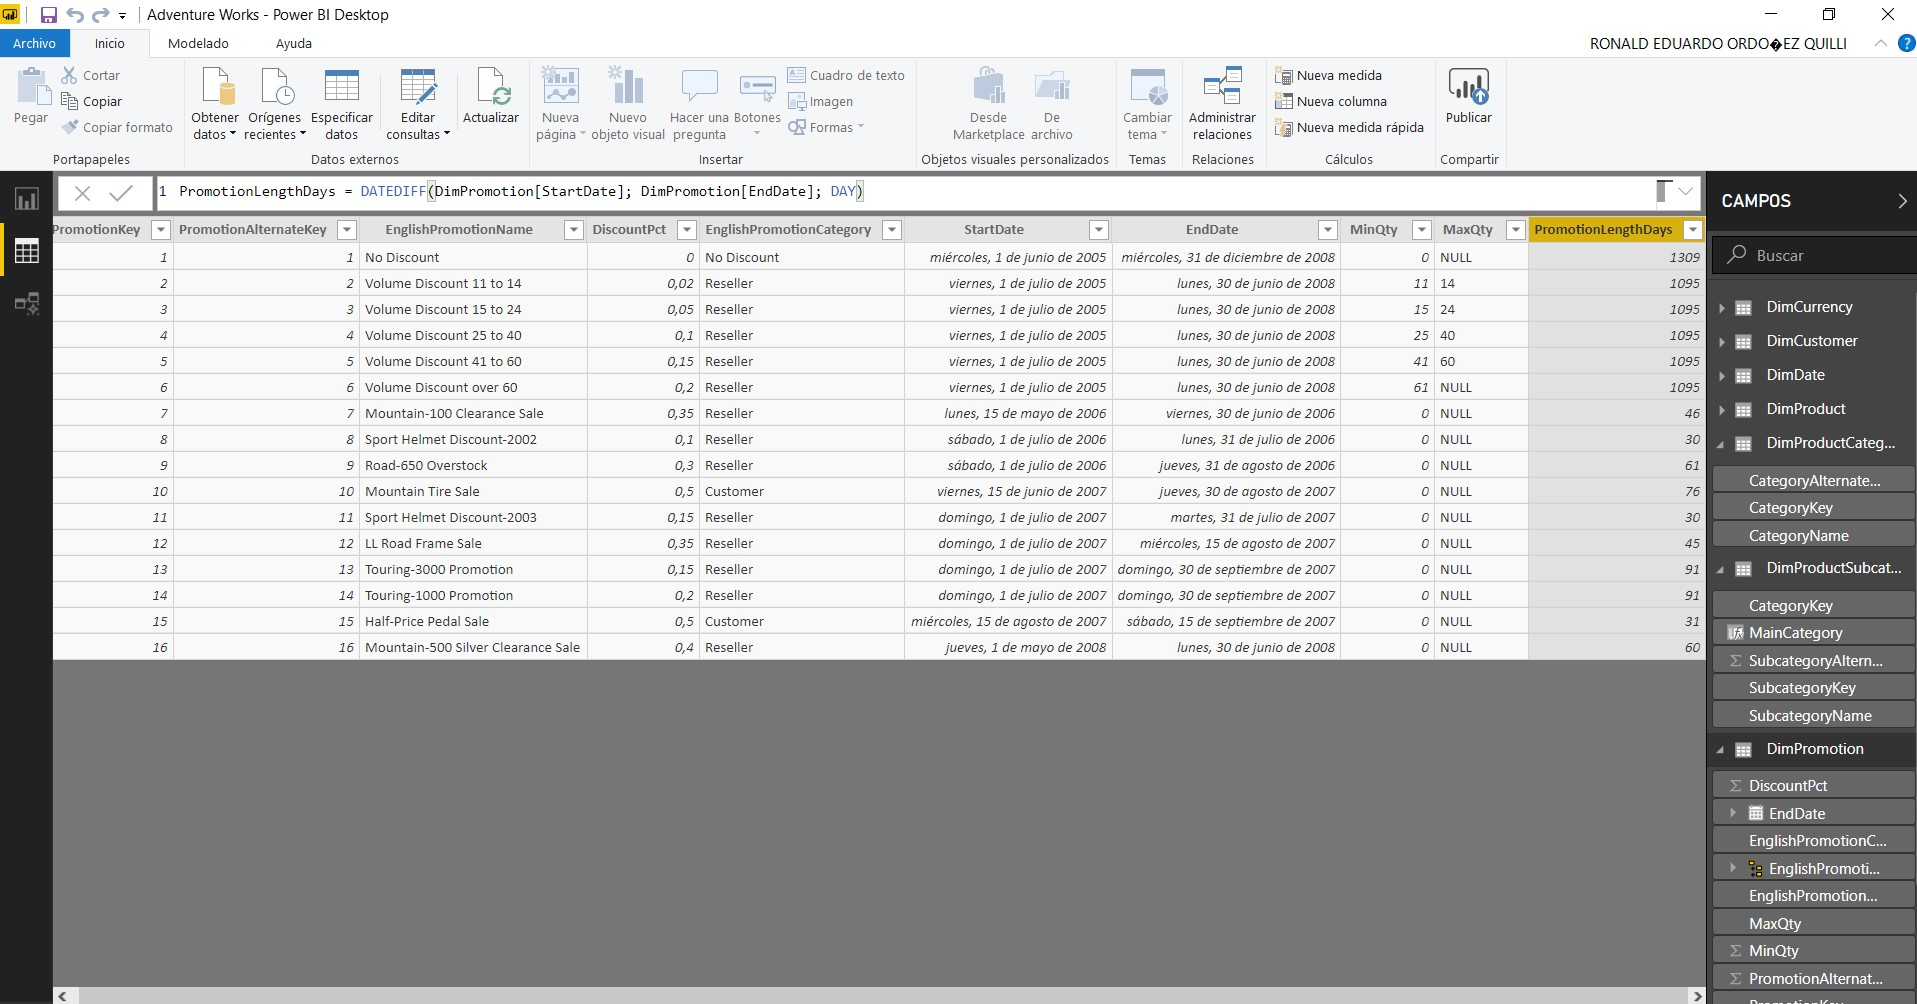
\includegraphics[width=16cm]{./Imagenes/imgpbi4} 
	\end{center}
	\begin{center}
	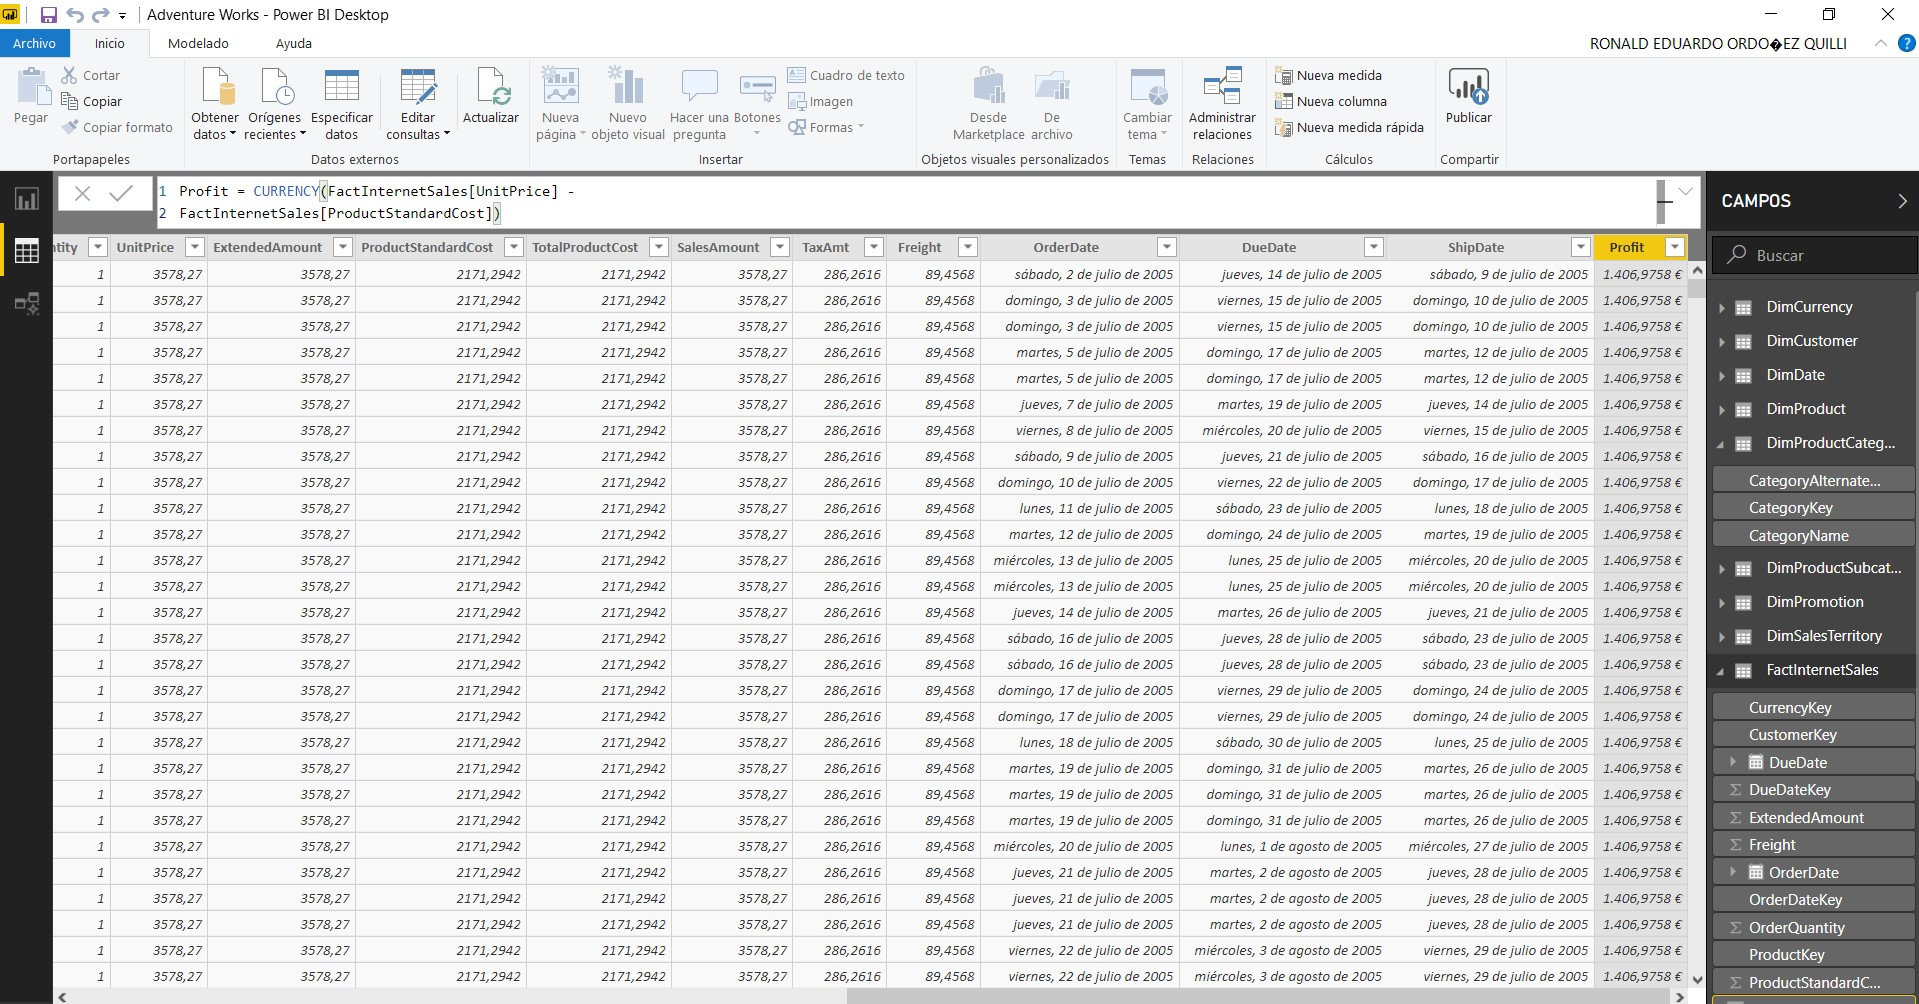
\includegraphics[width=16cm]{./Imagenes/imgpbi5} 
	\end{center}
	\item Informe en PowerBI
	\begin{center}
	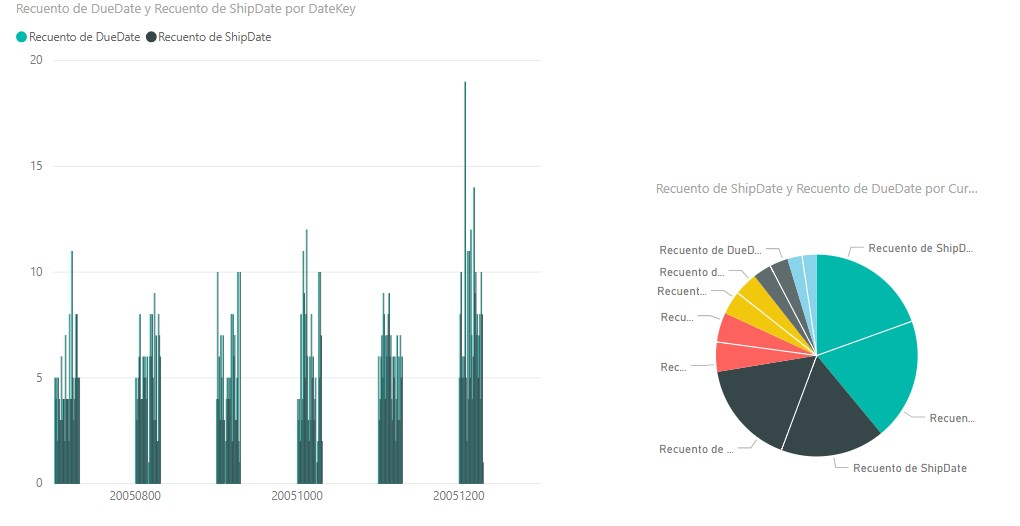
\includegraphics[width=16cm]{./Imagenes/imgpbi2} 
	\end{center}

Ruta del informe en el Power BI
\\
\url{https://app.powerbi.com/groups/me/reports/1a5e9816-31a8-46e2-b401-47d6bfac7293?ctid=b6b466ee-468d-4011-b9fc-fbdcf82ac90a} 
\end{itemize} 